\documentclass[main.tex]{subfiles}

\begin{document}

\chapter{Point Location}

Neste capítulo analisaremos uma variação do problema Point Location~\cite{SarnakT1986}, e mostraremos uma solução utilizando a ABB persistente descrita no capítulo~\ref{cap:rubronegra_persist}.

Dado um conjunto de polígonos~${\{P_1, \ldots, P_n\}}$ tal que nenhum dos polígonos se intersecta, queremos responder múltiplas consultas do seguinte tipo: Dado um ponto~$p$, determine~$i$ tal que~${p \in P_i}$ ou diga que tal~$i$ não existe.

Observe a Figura~\ref{fig:exemplo_pl}, ela mostra um exemplo do problema com 3 polígonos. Os pontos de consulta estão coloridos com a cor do polígono a qual pertencem, ou pretos se não pertencem a nenhum dos polígonos.



\begin{figure}
\centering
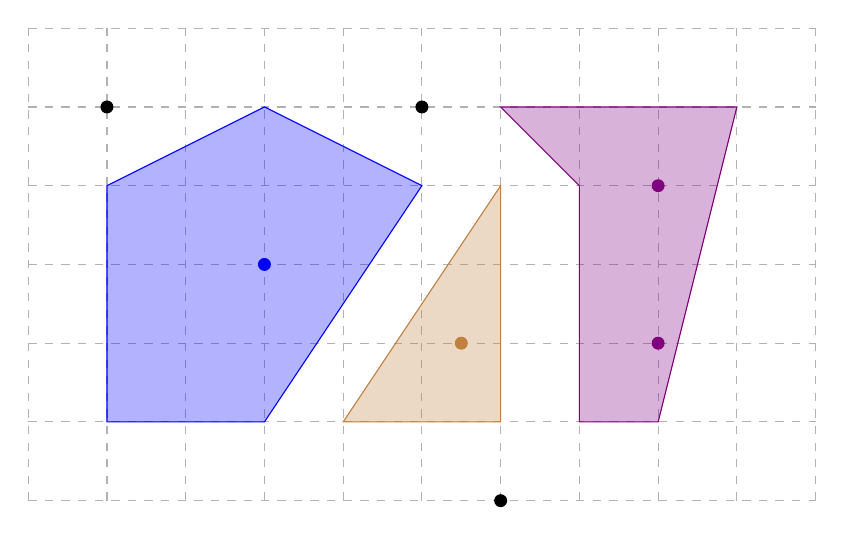
\begin{tikzpicture}[]

\newcounter{size}
\newcommand\polyg[2]{
	\setcounter{size}{0}
	\foreach \point [count=\i] in #1 {
		\stepcounter{size}
		\node[coordinate] (p1-\i) at \point {};
	}
	\fill[#2, opacity=0.3] (p1-1) \foreach \i in {2, ..., \value{size}} {-- (p1-\i)} -- cycle;
	\draw[#2, opacity=1] (p1-1) \foreach \i in {2, ..., \value{size}} {-- (p1-\i)} -- cycle;
}

\draw[opacity=0.3, dashed] (-8, 0) grid (2, 6);

\polyg {{(-7, 4), (-5, 5), (-3, 4), (-5, 1), (-7, 1)}}{blue};
\polyg {{(-2, 5), (-1, 4), (-1, 1), (0, 1), (1, 5)}}{violet};
\polyg {{(-2, 4), (-4, 1), (-2, 1)}}{brown};

\newcommand\drawpts[2]{ \foreach \point in #1 { \draw[fill=#2, color=#2] \point circle (0.075); }}

\drawpts{{(-5, 3)}}{blue};
\drawpts{{(-2.5, 2)}}{brown};
\drawpts{{(0, 4), (0, 2)}}{violet};
\drawpts{{(-3, 5), (-7, 5), (-2, 0)}}{black};

\end{tikzpicture}
\caption{Exemplo do problema descrito.} \label{fig:exemplo_pl}
\end{figure}

\end{document}
